\renewcommand{\thechapter}{5}
\chapter{Electronic Noise Measurements}
\label{ch:NoiseMeasurements}

We have described in chapter~\ref{ch:DenoisingTheory} the principles and algorithm behind denoising.  Among the points it makes is that a detailed noise model is required to perform denoising.  Equation~\ref{eq:FirstStatementOfNoiseCorrelations} specifies that the correlations in electronic noise are taken as inputs to denoising; in this chapter we describe the measurement of the electronic noise correlations.  Section~\ref{sec:NoiseCorrelationsMath}specifies the desired measurement; section~\ref{sec:NoiseCorrelationsTimeWindows} identifies the time-dependent behavior of noise; and section~\ref{sec:NoiseCorrelationsImplementation} describes the algorithm to measure noise from data.  We conclude in section~\ref{sec:NoiseCorrelationsFuture} with some possible future work to improve the quality of the noise measurements or use them in other aspects of the EXO-200 analysis.

\section{Mathematical Framework for Noise Correlations}\label{sec:NoiseCorrelationsMath}

A waveform on channel $i$ with no pulse on it consists entirely of a noise function $N_i[\tau]$.  The noise is a random function:  its value at each time $\tau$ is a random variable.  Our goal is to describe the joint probability distribution of those random variables.  Noise on different channels is correlated, so our joint probability distribution should describe not only the noise for all time samples $\tau$ on a particular channel $i$, but also the relation between noise on any distinct pair of channels $i$ and $j$.

We can guarantee that the noise is stationary because the waveforms are all subject to shaping which removes low-frequency noise components, as described in section~\ref{sec:DetectorReadout}.  It is conventional to study stationary noise in Fourier space.  This often leads to sharper features because noise often originates from environmental factors which demonstrate periodic behavior: in EXO-200, examples of possible sources of periodic waveform noise include acoustic noise from the cleanroom, mechanical vibrations of the various wires under tension in the TPC, or switching noise from the digital power supplies.  The Fourier transform also can lead to a simpler characterization of noise correlations: in a steady-state environment it is impossible for noise at two different frequencies to be correlated because the inner product of two sinusoidal functions with different frequencies is always zero.

We write the discrete Fourier transform of $N_i[\tau]$ as $\widetilde{N}_i[f]$, consistent with the notation described in section~\ref{sec:DenoisingNotationSetup}.  Although the specific choice of convention will not matter for any of the analysis in this work, for completeness we specify explicitly the definition of the discrete Fourier transform and its inverse as
\begin{align}
\widetilde{N}_i[f] &= \sum_{\tau = 0}^{T-1} N_i[\tau] e^{-2\pi \tau f \mathrm{i}/T}\label{eqn:NoiseChapterDefnFourierTransform}\\
N_i[\tau] &= \frac{1}{T}\cdot \sum_{f = 0}^{T-1} \widetilde{N}_i[f] e^{2\pi \tau f \mathrm{i}/T},
\end{align}
where $T$ is the (unitless) number of samples in the time domain waveform.  Both of these waveforms are assumed to be periodic, so we store $N[\tau]$ with $\tau \in [0, T)$ and $\widetilde{N}[f]$ with $f \in \left[0, \lfloor \frac{T}{2} \rfloor\right]$, where $\lfloor\,\rfloor$ indicates that rounding is performed downward.  This set of conventions matches the conventions of the real-to-complex discrete Fourier transform implemented by the popular FFTW library, which is available on all major computational platforms~\cite{FFTW05}.

Our sampling frequency of 1 MHz means that we can associate $\widetilde{N}_i[f]$ with noise at a frequency of $f/T$ MHz (where we again recall that $T$ and $f$ are unitless).  The accuracy of this association is dependent on the accuracy of the nominal 1 MHz sampling.  This is controlled by a nominal 80 MHz oscillator in the master TEM unit; preliminary investigations indicate that this frequency changes over time, and may deviate from a true 80 MHz period by as much as ten parts per million~\cite{DAQWeirdDetails,EXOElectronicsFunctionalSpecification}.  Since we apply low-pass filters with a combined effective cutoff frequency around 167 kHz, as described in section~\ref{sec:DetectorReadout}, this is expected to have a negligible effect on our noise measurements.

To quantify the second moments of the noise, we have seen in equation~\ref{eqn:SystemToSolve} that it will be useful to measure expectation values of the real-valued quantities for each pair of channels $i$, $j$ and each frequency index $f$:
\begin{subequations}\label{eq:NoiseChapterAllExpValues}\begin{align}
&\left<\widetilde{N}^R_i[f]\widetilde{N}^R_j[f]\right>\label{eq:NoiseChapterFirstExpValue}\\
&\left<\widetilde{N}^R_i[f]\widetilde{N}^I_j[f]\right>\label{eq:NoiseChapterSecondExpValue}\\
&\left<\widetilde{N}^I_i[f]\widetilde{N}^I_j[f]\right>\label{eq:NoiseChapterThirdExpValue},
\end{align}\end{subequations}
where $\widetilde{N}^R$ and $\widetilde{N}^I$ denote the real and imaginary parts of the noise in Fourier space, respectively.

We can see that equations~\ref{eq:NoiseChapterAllExpValues} possess some symmetries which may reduce the size of a file and permit the exploitation of faster matrix operations.  First, equations~\ref{eq:NoiseChapterFirstExpValue} and \ref{eq:NoiseChapterThirdExpValue} are symmetric under exchange of channel indices $i$ and $j$, so we can store these values on disk more compactly by only storing the expectation values where $i \leq j$.

A second symmetry comes from the observation that for most frequencies the phase is random because a waveform trigger time is uncorrelated with the phase of any noise frequency.  More specifically, we can decompose $\widetilde{N}[f]$ into a real-valued amplitude $A[f]$ and phase $\theta[f]$ by
\begin{equation}
\widetilde{N}[f] = A[f]e^{\theta[f] \mathrm{i}}.
\end{equation}
The phase and amplitude cannot be correlated because the phase depends solely on where we choose to sample a waveform from the detector, whereas the amplitude at a particular frequency is constant in time.  By the Nyquist-Shannon sampling theorem (see for example~\cite{659497}) we can reconstruct this function unambiguously for all frequencies less than half of the sampling rate; in our case, we can reconstruct perfectly all parameters for $f < T/2$.  This means that in a waveform with odd-valued $T$ we can perfectly reconstruct all components, and in a waveform with even-valued $T$ we can perfectly reconstruct all components except $f = T/2$.

For the frequency $f = T/2$ in an even-length time-domain waveform, we cope with the ambiguous reconstruction of $A[T/2]$ and $\theta[T/2]$ by asserting that $\theta[T/2]$ is zero, so that the last Fourier coefficient is strictly real-valued; this comes automatically from equation~\ref{eqn:NoiseChapterDefnFourierTransform}.  Additionally, for the zero-frequency component $\theta[0] = 0$ is enforced by the fact that $N[\tau]$ is real-valued.  In all other frequency components, however, there is a unique choice of $\theta[f] \in [0,2\pi)$, and it can have no directional preference because the time of the event trigger has no preference.  Put another way, for some fixed time $\tau_0$ it is equally likely that we sample a waveform starting at $\tau_0$, $\tau_0 + 1$, ..., each of which would result in a different phase $\theta[f]$.  This can also be viewed as a symmetry of the noise: if we translate the time of the waveform we sample, it has the effect of rotating the phase $\theta[f]$.  All expectation values should be invariant under such an action.

We can then expand equation~\ref{eq:NoiseChapterFirstExpValue}, taking (as discussed earlier) only the phase to be random:
\begin{align}
\left<\widetilde{N}^R_i[f]\widetilde{N}^R_j[f]\right> &= \left<A_i[f]A_j[f] cos\left(\theta_i[f]\right)cos\left(\theta_j[f]\right)\right> \\
  &= \left<A_i[f]A_j[f]\right> \cdot \frac{\left<cos\left(\theta_i[f] + \theta_j[f]\right) + cos\left(\theta_i[f] - \theta_j[f]\right)\right>}{2}.\\
\intertext{We can see that $\theta_i[f] + \theta_j[f]$ is not invariant under time translation; as a result, we can assert that the left term must have an expectation value equal to zero.  On the other hand, $\theta_i[f] - \theta_j[f]$ is invariant under time translation, so that term can survive:}
\left<\widetilde{N}^R_i[f]\widetilde{N}^R_j[f]\right> &= \frac{\left<A_i[f]A_j[f]\right>}{2} \cdot \left<cos\left(\theta_i[f] - \theta_j[f]\right)\right>.\label{eqn:NoiseChapterPhaseEqnOne}\\
\intertext{Similarly for the other expectation values:}
\left<\widetilde{N}^R_i[f]\widetilde{N}^I_j[f]\right> &= \frac{\left<A_i[f]A_j[f]\right>}{2} \cdot \left<sin\left(\theta_j[f] - \theta_i[f]\right)\right>\label{eqn:NoiseChapterPhaseEqnTwo}\\
\left<\widetilde{N}^I_i[f]\widetilde{N}^I_j[f]\right> &= \frac{\left<A_i[f]A_j[f]\right>}{2} \cdot \left<cos\left(\theta_i[f] - \theta_j[f]\right)\right>.\label{eqn:NoiseChapterPhaseEqnThree}
\end{align}

We can see from equations~\ref{eqn:NoiseChapterPhaseEqnOne}-\ref{eqn:NoiseChapterPhaseEqnThree} that for frequencies other than $0$ and $T/2$, the following identities hold:
\begin{align}
\left<\widetilde{N}^R_i[f]\widetilde{N}^R_j[f]\right> &= \left<\widetilde{N}^I_i[f]\widetilde{N}^I_j[f]\right> \label{eqn:NoiseSymmetryRRII}\\
\left<\widetilde{N}^R_i[f]\widetilde{N}^I_j[f]\right> &= -\left<\widetilde{N}^R_j[f]\widetilde{N}^I_i[f]\right>.\label{eqn:NoiseSymmetryRIRI}
\end{align}

Taking advantage of these symmetries, we can compute that for $71$ channels and waveforms containing $2048$ samples we need to store roughly five million independent values to characterize the noise correlations; this results in a file of size roughly $40$ megabytes for each snapshot of the noise correlations.  We show in section~\ref{sec:NoiseCorrelationsTimeWindows} that only a small number of snapshots appear to be necessary, so this can be a manageable dataset.

\section{Time Windows of Constant Noise}\label{sec:NoiseCorrelationsTimeWindows}

Section~\ref{sec:NoiseCorrelationsMath} has described the noise correlation information which denoising requires and demonstrated that a snapshot of the noise will require roughly 40 MB of data.  Although EXO-200 has a significant amount of noise information available and is capable of producing a detailed history of the noise variations in time, taking such an approach would quickly produce an unmanageable quantity of data.  This section explains how the noise behavior appears to be stable for long periods of time, permitting us to create a coarse-grained history of the noise without losing significant accuracy.

The approach to identifying these constant-noise time windows is two-fold.  Firstly, we identify certain environmental changes which are likely to have a significant impact on the noise observed on the APDs.  Since the times at which these changes occur are generally known precisely (and usually fall between runs), we can place time boundaries accurately when an environmental change is traced as the origin of a change.

Secondly, we develop a set of parameters which can easily be viewed in plots versus time.  These trend plots are then reviewed qualitatively by collaboration members, and stepwise changes in any of these parameters can be interpreted as a change in detector noise at the time of the step.  Although sometimes it is necessary to guess the precise time when a change in noise occurred, when possible we review the environmental conditions of the detector in more detail and search for possible causes for the change in noise which would permit us to pinpoint the time of the change.

\begin{figure}
\begin{center}
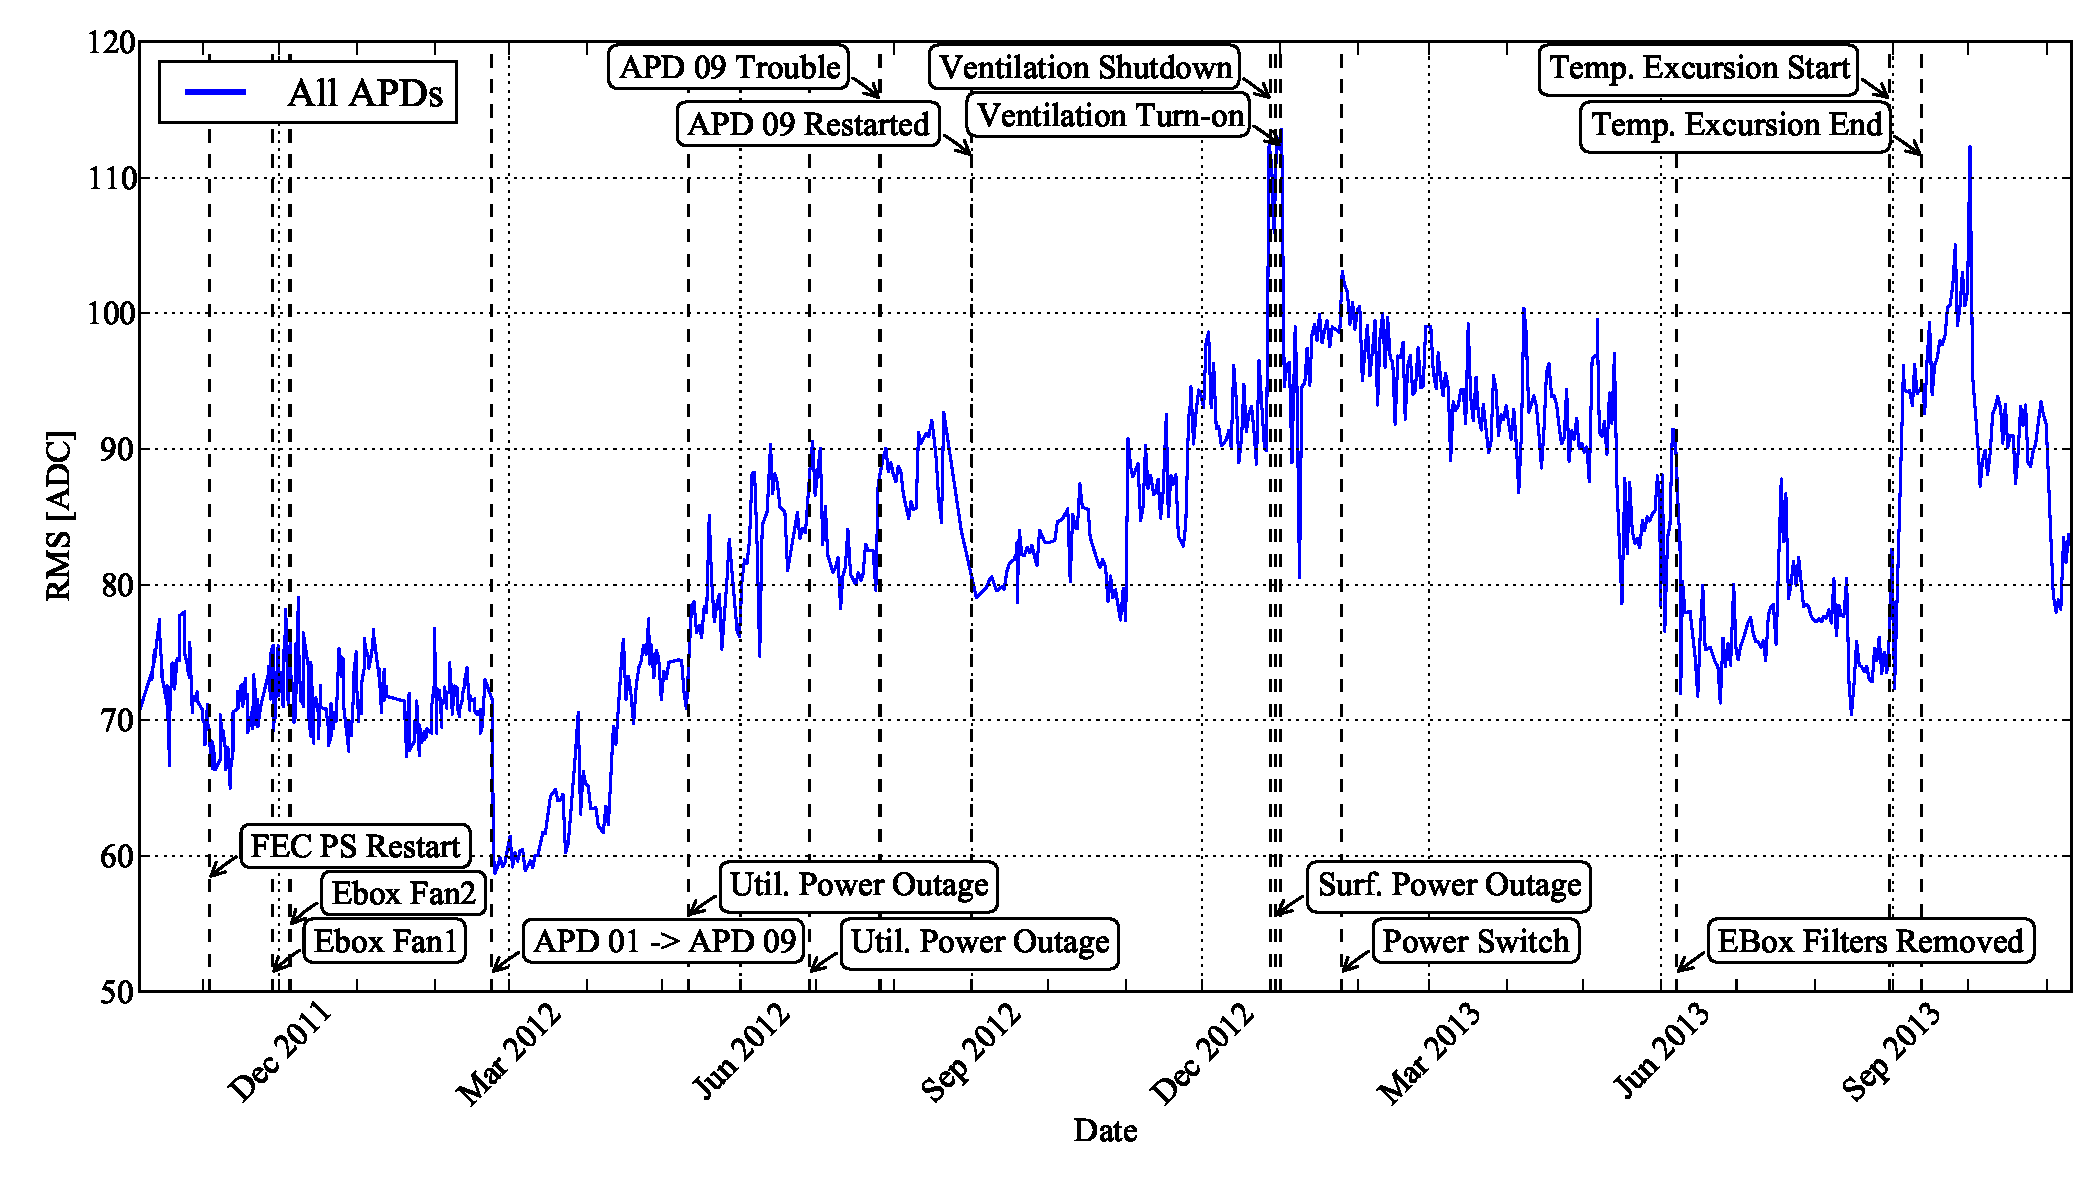
\includegraphics[keepaspectratio=true,width=\textwidth]{APDNoiseVsActions_sumall.pdf}
\end{center}
\renewcommand{\baselinestretch}{1}
\small\normalsize
\begin{quote}
\caption{Sum noise for all APD channels measured from charge injection runs, with environmental changes indicated which may correlate with observed changes in noise.  Data provided by Josiah Walton.}
\label{fig:APDSumAllNoise_JosiahEnvironmental}
\end{quote}
\end{figure}
\renewcommand{\baselinestretch}{2}
\small\normalsize

\begin{figure}
\begin{center}
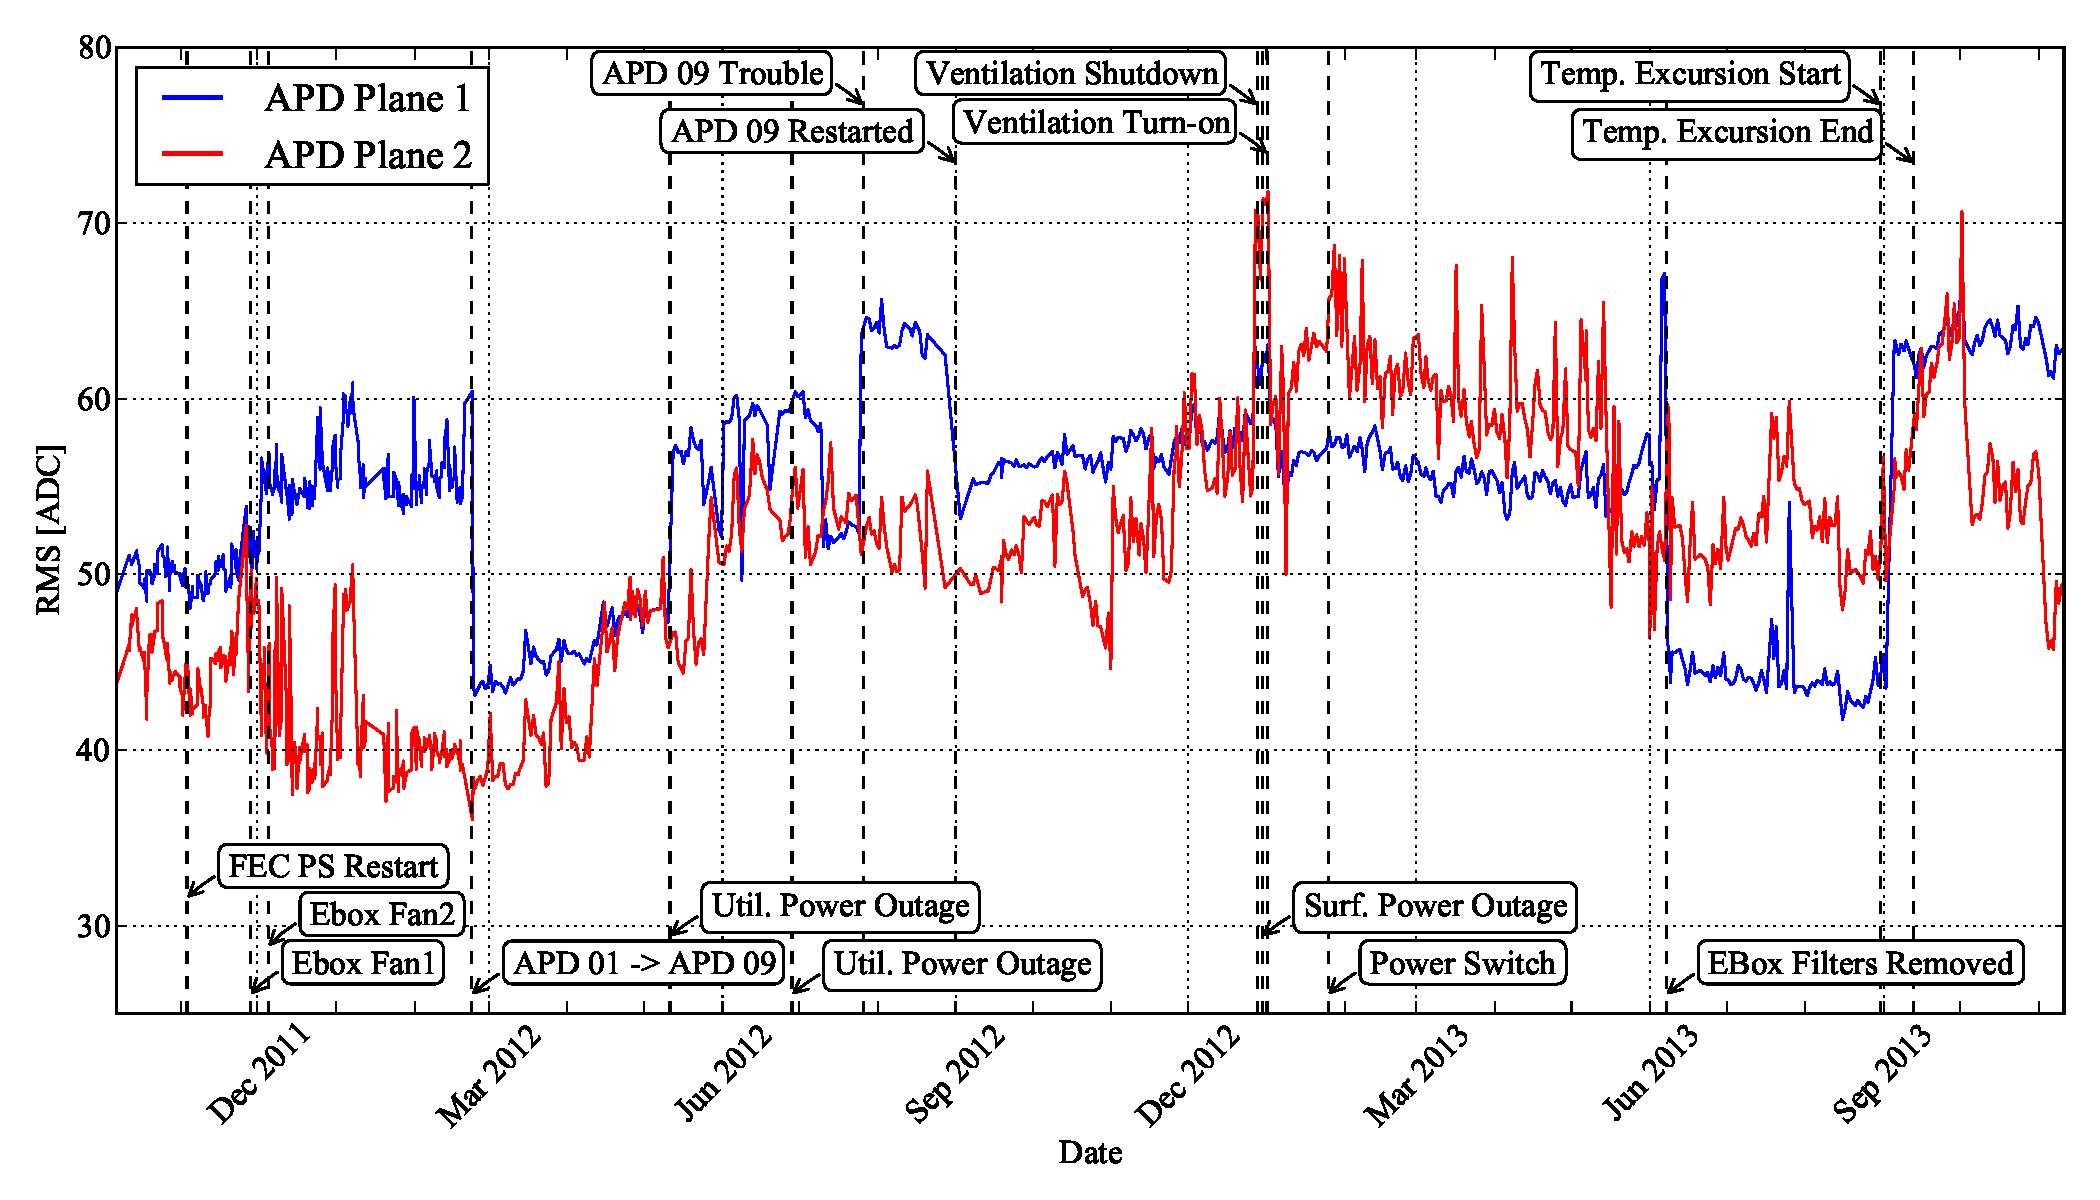
\includegraphics[keepaspectratio=true,width=\textwidth]{APDNoiseVsActions_planes.pdf}
\end{center}
\renewcommand{\baselinestretch}{1}
\small\normalsize
\begin{quote}
\caption{Sum noise for each APD plane measured from charge injection runs, with environmental changes indicated which may correlate with observed changes in noise.  Data provided by Josiah Walton.}
\label{fig:APDSumPlaneNoise_JosiahEnvironmental}
\end{quote}
\end{figure}
\renewcommand{\baselinestretch}{2}
\small\normalsize

\begin{figure}
\begin{center}
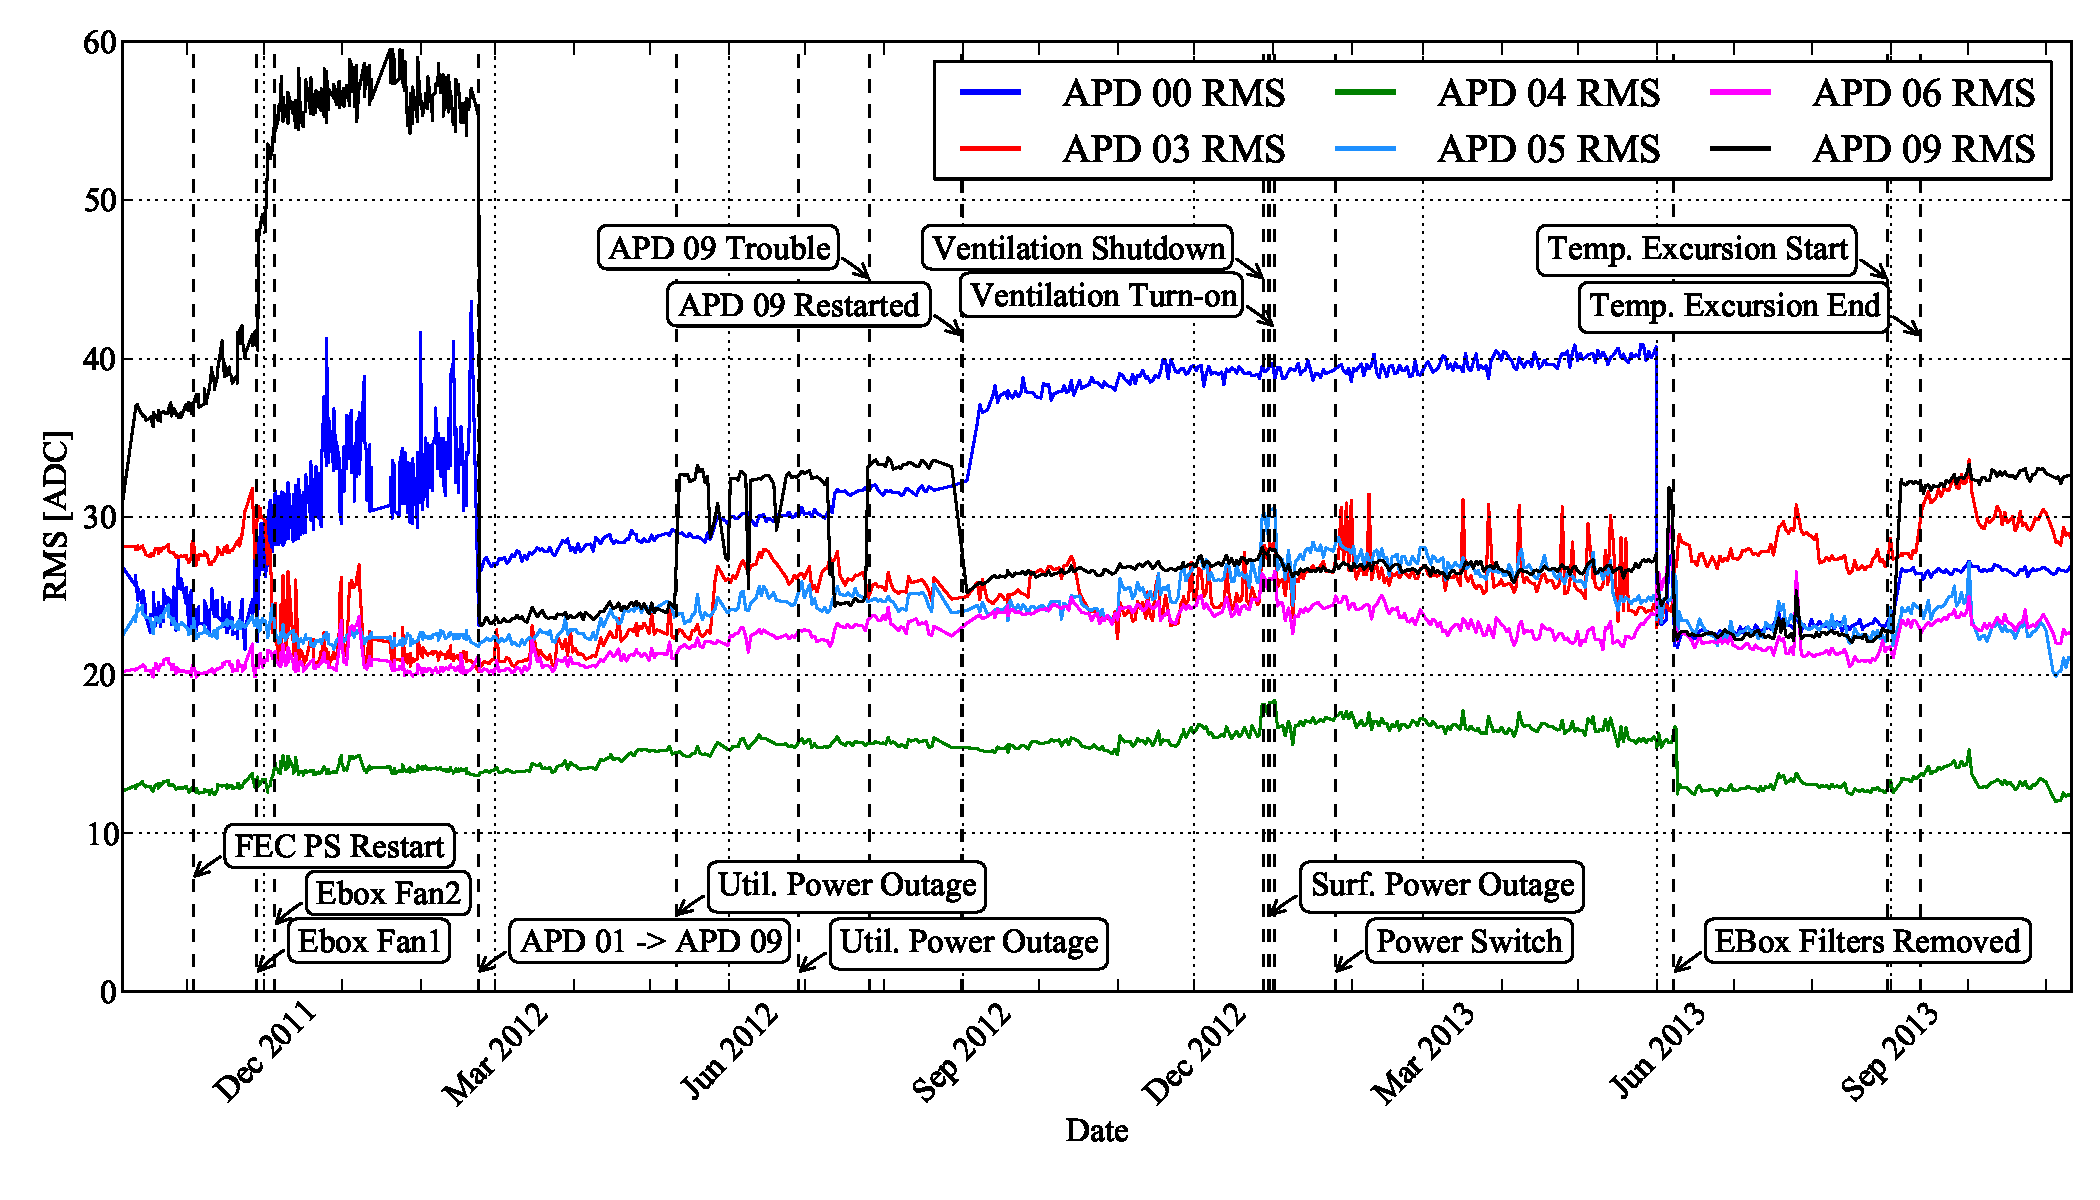
\includegraphics[keepaspectratio=true,width=\textwidth]{APDNoiseVsActions_boards.pdf}
\end{center}
\renewcommand{\baselinestretch}{1}
\small\normalsize
\begin{quote}
\caption{Sum noise for each APD electronics board measured from charge injection runs, with environmental changes indicated which may correlate with observed changes in noise.  Data provided by Josiah Walton.}
\label{fig:APDSumBoardNoise_JosiahEnvironmental}
\end{quote}
\end{figure}
\renewcommand{\baselinestretch}{2}
\small\normalsize

\begin{figure}
\begin{center}
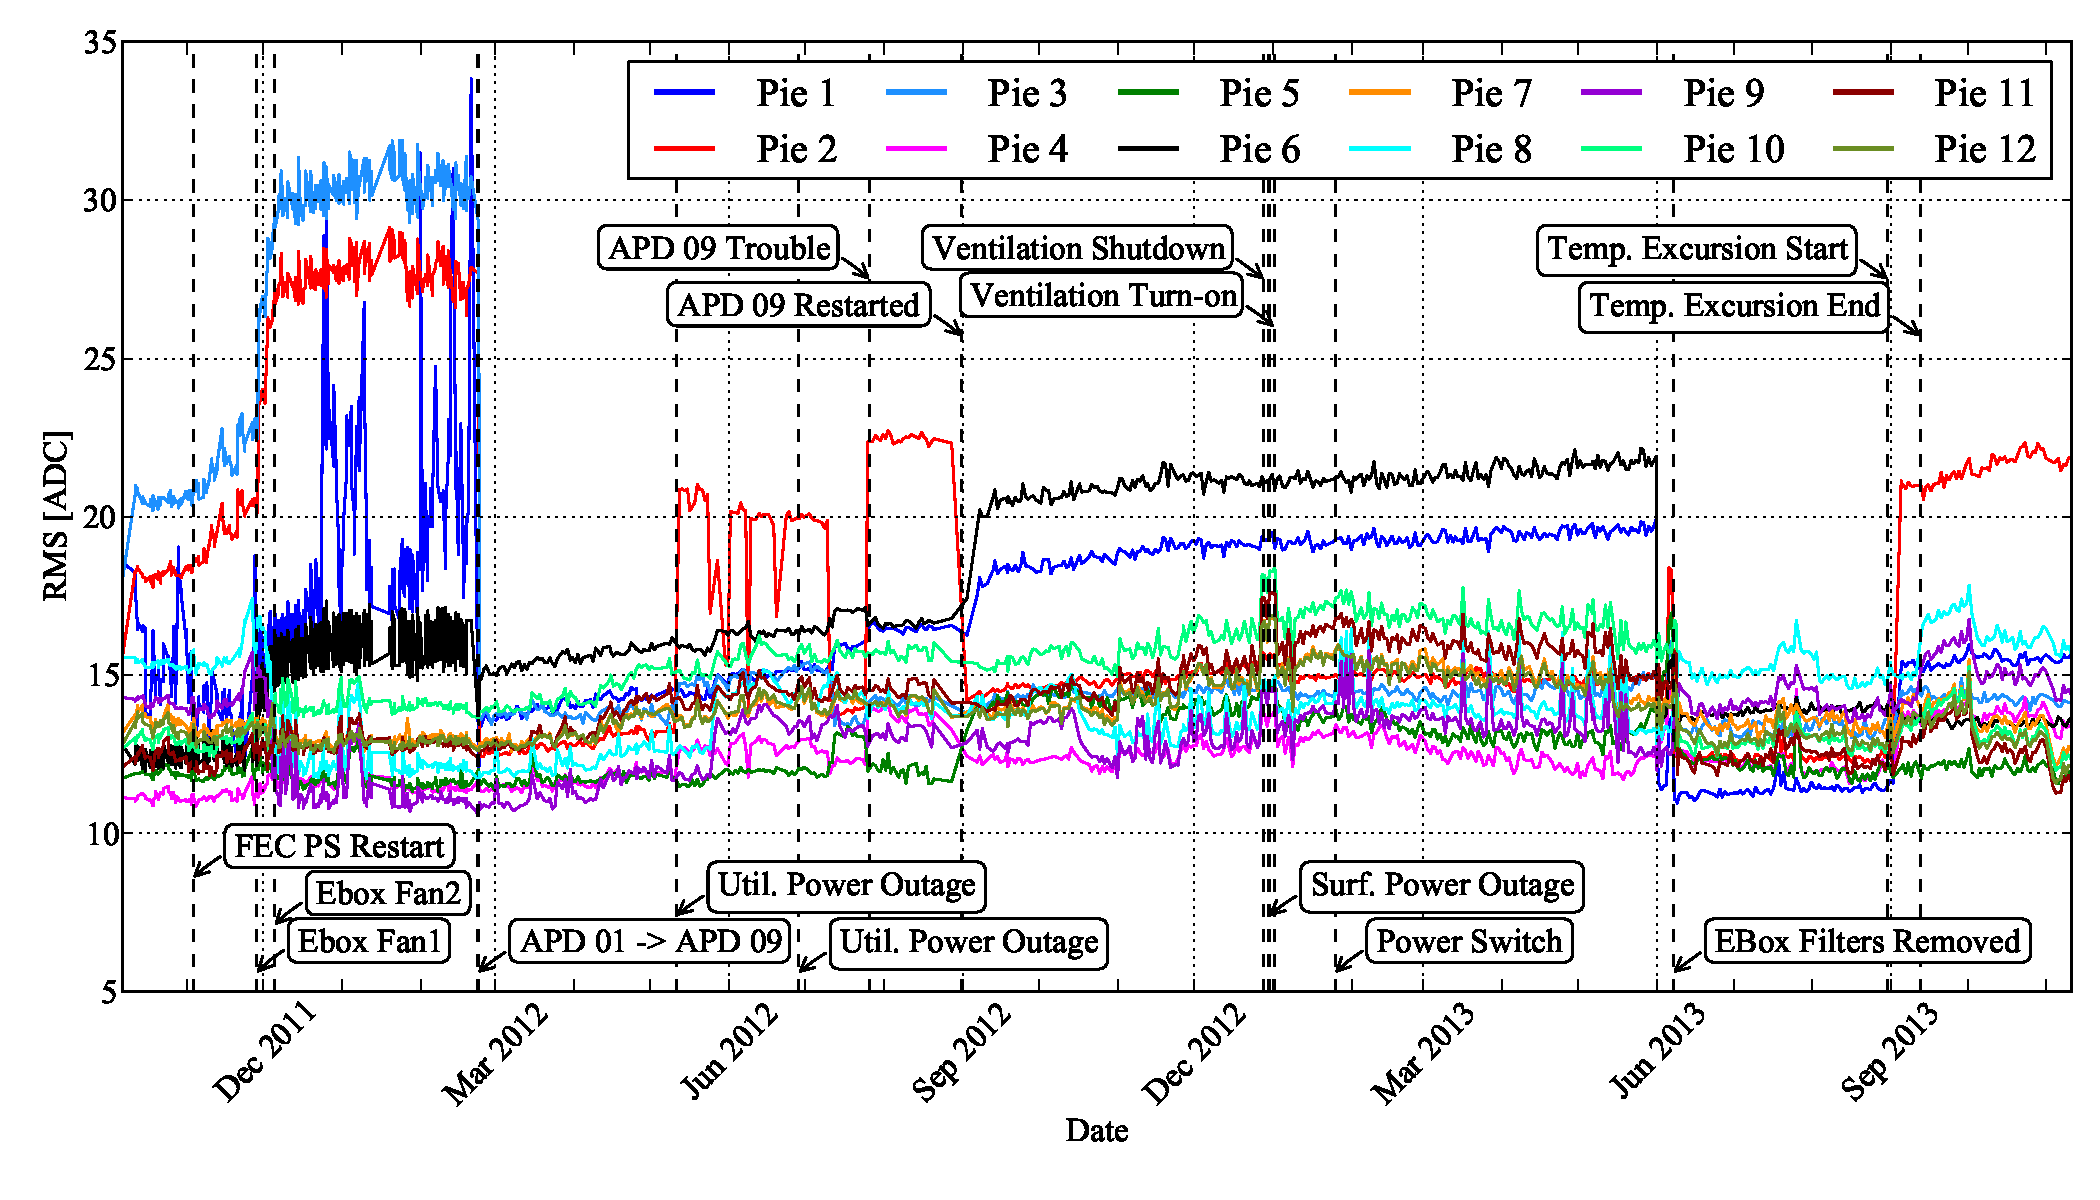
\includegraphics[keepaspectratio=true,width=\textwidth]{APDNoiseVsActions_pies.pdf}
\end{center}
\renewcommand{\baselinestretch}{1}
\small\normalsize
\begin{quote}
\caption{Sum noise for each APD pie (6-7 channels) measured from charge injection runs, with environmental changes indicated which may correlate with observed changes in noise.  Data provided by Josiah Walton.}
\label{fig:APDSumPieNoise_JosiahEnvironmental}
\end{quote}
\end{figure}
\renewcommand{\baselinestretch}{2}
\small\normalsize

\begin{figure}
\begin{center}
\includegraphics[keepaspectratio=true,page=6,width=\textwidth,clip=true,trim=0.2in 0.5in 0.5in 0.3in]{APD_Denoising_noise_correlations.pdf}
\end{center}
\renewcommand{\baselinestretch}{1}
\small\normalsize
\begin{quote}
\caption{Time trend of $\left<\widetilde{N}^R_{192}[385]\widetilde{N}^R_{193}[385]\right>$ (black), $\left<\widetilde{N}^R_{192}[385]\widetilde{N}^I_{193}[385]\right>$ (green), and $\left<\widetilde{N}^I_{192}[385]\widetilde{N}^I_{193}[385]\right>$ (red) corresponding to the correlations between channels 192 and 193 at 188 kHz.  Blue lines indicate tentative noise windows~\cite{MikeCoherentAPDNoise}.}
\label{fig:MikeNoise_192_193}
\end{quote}
\end{figure}
\renewcommand{\baselinestretch}{2}
\small\normalsize

\begin{figure}
\begin{center}
\includegraphics[keepaspectratio=true,page=5,width=\textwidth,clip=true,trim=0.2in 0.5in 0.5in 0.3in]{APD_Denoising_noise_correlations.pdf}
\end{center}
\renewcommand{\baselinestretch}{1}
\small\normalsize
\begin{quote}
\caption{Time trend of $\left<\widetilde{N}^R_{202}[383]\widetilde{N}^R_{203}[383]\right>$ (black), $\left<\widetilde{N}^R_{202}[383]\widetilde{N}^I_{203}[383]\right>$ (green), and $\left<\widetilde{N}^I_{202}[383]\widetilde{N}^I_{203}[383]\right>$ (red) corresponding to the correlations between channels 202 and 203 at 187 kHz.  Blue lines indicate tentative noise windows~\cite{MikeCoherentAPDNoise}.}
\label{fig:MikeNoise_202_203}
\end{quote}
\end{figure}
\renewcommand{\baselinestretch}{2}
\small\normalsize

\begin{table}
\begin{singlespace}
\begin{center}
\begin{tabular}{|c|c|p{.52\textwidth}|}\hline
Runs & Dates & Comments \\\hline
2401-2423 & 9/28/2011-9/30/2011 & APDs biased to special ``9-28-11'' settings. \\\hline
2424-2690 & 9/30/2011-11/2/2011 & FEC voltage adjustment on 11/2/2011. \\\hline
2691-2852 & 11/2/2011-11/28/2011 & Cooling fan installed on Ebox 1, 11/28/2011. \\\hline
2853-2891 & 11/28/2011-12/4/2011 & Cooling fan installed on Ebox 2, 12/4/2011. \\\hline
2892-3117 & 12/4/2011-1/13/2012 & Power outage, no data 1/13-1/19. \\\hline
3118-3326 & 1/13/2012-2/23/2012 & During runs 3314-3320 (2/22) APD channel 163 was disconnected.  During runs 3324-3331 (2/23) front-end cards were swapped.\\\hline
3327-3700 & 2/23/2012-5/11/2012 & Brief power outage on 5/11. \\\hline
3701-3933 & 5/11/2012-7/10/2012 & Possibly associated with a TEM temperature spike on the morning of 7/10; cause not known. \\\hline
3934-4003 & 7/10/2012-7/24/2012 & Possibly associated with a new TEM module on 7/24. \\\hline
4004-4126 & 7/24/2012-8/28/2012 & Power outage, no data 8/28-8/30, messy recovery of APD01. \\\hline
4127-4589 & 8/28/2012-12/27/2012 & Pump reset on 12/27, but it is not clear this is the cause of the short spike in APD noise. \\\hline
4590-4609 & 12/27/2012-1/1/2013 & As mysteriously as the noise came on 12/27, it disappeared sometime between 1/1 and 1/2. \\\hline
4609-4779 & 1/1/2013-2/20/2013 & Not clear that anything happened on 2/20; we should review this boundary to ensure it is significant. \\\hline
4780-5061 & 2/20/2013-5/14/2013 & Noise on TPC2 changed sometime around 5/14-5/20.  Thermal stores stopped cooling on the evening of 5/17, but it it unclear how this would impact the APDs. \\\hline
5062-5197 & 5/14/2013-6/7/2013 & Modifications to electronics boards on 6/7. \\\hline
5198-5590 & 6/7/2013-8/31/2013 & Temperature excursions in the cleanroom around 8/31 permanently impacted the APD behavior. \\\hline
5591-5892 & 8/31/2013-11/11/2013 & Differential-pressure excursion on 11/11. \\\hline
\end{tabular}
\end{center}
\end{singlespace}
\caption{Recommended noise windows, based on the current understanding of changes in noise and their possible causes.  This is not the same as the noise windows actually used in the present analysis; for those, please see table~\ref{tab:NoiseWindowsUsedThisAnalysis}.}
\label{tab:NoiseWindowsRecommendedForFuture}
\end{table}

\begin{table}
\begin{singlespace}
\begin{center}
\begin{tabular}{|c|c|}\hline
Runs & Dates \\\hline
2401-2423 & 9/28/2011-9/30/2011 \\\hline
2424-2690 & 9/30/2011-11/2/2011 \\\hline
2691-2852 & 11/2/2011-11/28/2011 \\\hline
2853-2891 & 11/28/2011-12/4/2011 \\\hline
2892-3117 & 12/4/2011-1/13/2012 \\\hline
3118-3326 & 1/13/2012-2/23/2012 \\\hline
3327-3700 & 2/23/2012-5/11/2012 \\\hline
3701-3949 & 5/11/2012-7/12/2012 \\\hline
3950-4140 & 7/12/2012-9/2/2012 \\\hline
4141-4579 & 9/2/2012-12/24/2012 \\\hline
4580-4779 & 12/24/2012-2/20/2013 \\\hline
4780-5197 & 2/20/2013-6/7/2013 \\\hline
5198-5590 & 6/7/2013-8/31/2013 \\\hline
5591-5892 & 8/31/2013-11/11/2013 \\\hline
\end{tabular}
\end{center}
\end{singlespace}
\caption{Noise windows used for the current analysis.  For the noise windows recommended for future analyses and a more detailed explanation of the causes of changes in noise behavior, see table~\ref{tab:NoiseWindowsRecommendedForFuture}.}
\label{tab:NoiseWindowsUsedThisAnalysis}
\end{table}

One source of noise information is provided from charge injection runs.  These runs have been taken daily for the entire history of our dataset, and are designed to inject a known pulse half-way through the 2048-sample waveform.  Since the pulse time is known, it is also generally true that the pretrace has no pulse on it and can be viewed as a pure noise sample.  It is possible by coincidence for a low-background event to deposit energy which is observed as a pulse in the pretrace, but this is extremely rare.

The approach described in~\cite{JosiahCoherentAPDNoise} is to use the pretrace samples between 200 and 800 $\mu$s from charge injection runs as noise samples.  A subset of waveforms -- APD pies, electronics boards, planes, or all APD channels together -- are summed together for each event, and the root-mean-square variation in the summed waveform is averaged over the samples between 200 and 800 $\mu$s and over all events in the charge injection run.  Each charge injection run contains 13,200 events, all of which can be used to improve the quality of this average root-mean-square measurement of noise on that subset of channels.

Figures~\ref{fig:APDSumAllNoise_JosiahEnvironmental}, \ref{fig:APDSumPlaneNoise_JosiahEnvironmental}, \ref{fig:APDSumBoardNoise_JosiahEnvironmental}, and \ref{fig:APDSumPieNoise_JosiahEnvironmental} show the noise for all APDs, APD planes, APD electronics boards, and APD pies respectively, with notable environmental changes overlaid to demonstrate their correlation with changes in noise.  These trending plots demonstrate that although the noise does undergo day-to-day fluctuations (possibly due to insufficient sample statistics in the charge injection runs) and some gradual changes over time, the dominant effects are from stepwise changes which are generally correlated with a change in the detector environment.

Another approach to understanding the behavior of noise with respect to time is to compute noise correlations $\left<\widetilde{N}^R_i[f]\widetilde{N}^R_j[f]\right>$, $\left<\widetilde{N}^R_i[f]\widetilde{N}^I_j[f]\right>$, and $\left<\widetilde{N}^I_i[f]\widetilde{N}^I_j[f]\right>$ for some particular choice of channels $i$ and $j$ and frequency $f$, and identify changes in those particular values over time.  The algorithm for computing these noise correlations will be described fully in section~\ref{sec:NoiseCorrelationsImplementation}; the philosophy is simply that it is difficult to visualize changes in a dataset of five million values, but easy to visualize changes in some very small subset of those values.  Changes in the small subset are expected to indicate changes in overall noise behavior; by sampling enough choices of $i$, $j$, and $f$ we can hope to identify all times when the noise behavior changed.

To guide this search, we focus our attention on known peaks in the noise power spectrum; furthermore, we focus on frequencies which have been observed to produce noise that is highly correlated across channels.  One example of such a noise peak is around 190 kHz, and examples of the trending of noise correlation values are shown in figures~\ref{fig:MikeNoise_192_193} and \ref{fig:MikeNoise_202_203}.  There we can see that the changes in noise correlations for a particular frequency and channel pair can be dramatic.  This method of understanding our noise seems to be a powerful and sensitive approach to complement studies based on root-mean-square noise measurements described earlier.

The currently recommended noise run windows are listed in table~\ref{tab:NoiseWindowsRecommendedForFuture}.  An attempt has also been made to identify the reasons for changes in noise behavior, but in some cases there is no clear change to the detector that is correlated with the change in noise.  Future work may include combining all sources of noise trending information to obtain a more precise understanding of exactly when the behavior change occurred.

The run windows recommended in table~\ref{tab:NoiseWindowsRecommendedForFuture} are recommended for future work; however, they differ in some instances from the run windows used for the present analysis.  These are listed in table~\ref{tab:NoiseWindowsUsedThisAnalysis}.  In some instances the change in run range is minor and comes from a closer examination of exactly when the noise behavior changed; in others, more careful analysis revealed additional stepwise changes to the noise which had not previously been observed.  The energy resolution achieved will be shown in section~\ref{sec:RotatedEnergyResMeasurement} to be fairly stable in time, so it is not believed that the present analysis was significantly impacted by these slight variations in choice of noise run windows, but this assertion has not been quantified.

Future work can continue to improve the choice of noise run windows.  One detail which is neglected in the present analysis is the selection of runs to be used within a run range.  In the present analysis, all low-background runs which were used in the final dataset are also used for noise measurements.  However, this may not always be ideal.

A specific example comes from runs 3321-3323, which occur after channel 163 was disconnected but before electronics boards were replaced.  It is not advisable in this case for so few runs to form their own noise window because the quantity of statistics would be insufficient, but retaining them in the noise window formed by runs 3118-3326 could bias our estimates of noise on channel 163.  Instead, those runs should not have been used to measure noise at all; this will be corrected in future work.

Additional studies may be necessary if denoising is extended to include the wire channels.  The wire noise is generally more stable than the APD noise~\cite{JosiahCoherentAPDNoise}.  However, there are exceptions to this observation; one known exception comes from the Spring of 2012, when u-wire channel 16 was mistakenly dropped from data acquisition.  If data prior to run 2464 is used in a future analysis, the change in u-wire electronics in early Fall 2011 would also need to be accounted for.

The most significant future work, though, simply consists of more careful study to characterize exactly when the noise behavior changed and whether slow changes in noise behavior may warrant the creation of additional time windows.  These investigations will feed into further improvements to denoising, but they may also inform a better understanding of the noise in our detector.  The current body of work already constitutes a rich set of studies performed by many collaboration members, and has enabled the use of a manageable set of noise files to characterize the whole history of our detector.

\section{Algorithm for Measuring Noise}\label{sec:NoiseCorrelationsImplementation}

For each of the noise windows specified in table~\ref{tab:NoiseWindowsUsedThisAnalysis}, it is necessary to locate a pool of ``clean'' events when no pulse occurred; these will be interpreted as samples of pure noise.  This section will describe the selection cuts for clean events, followed by the data format currently used to store noise correlation information.

\begin{figure}
\begin{center}
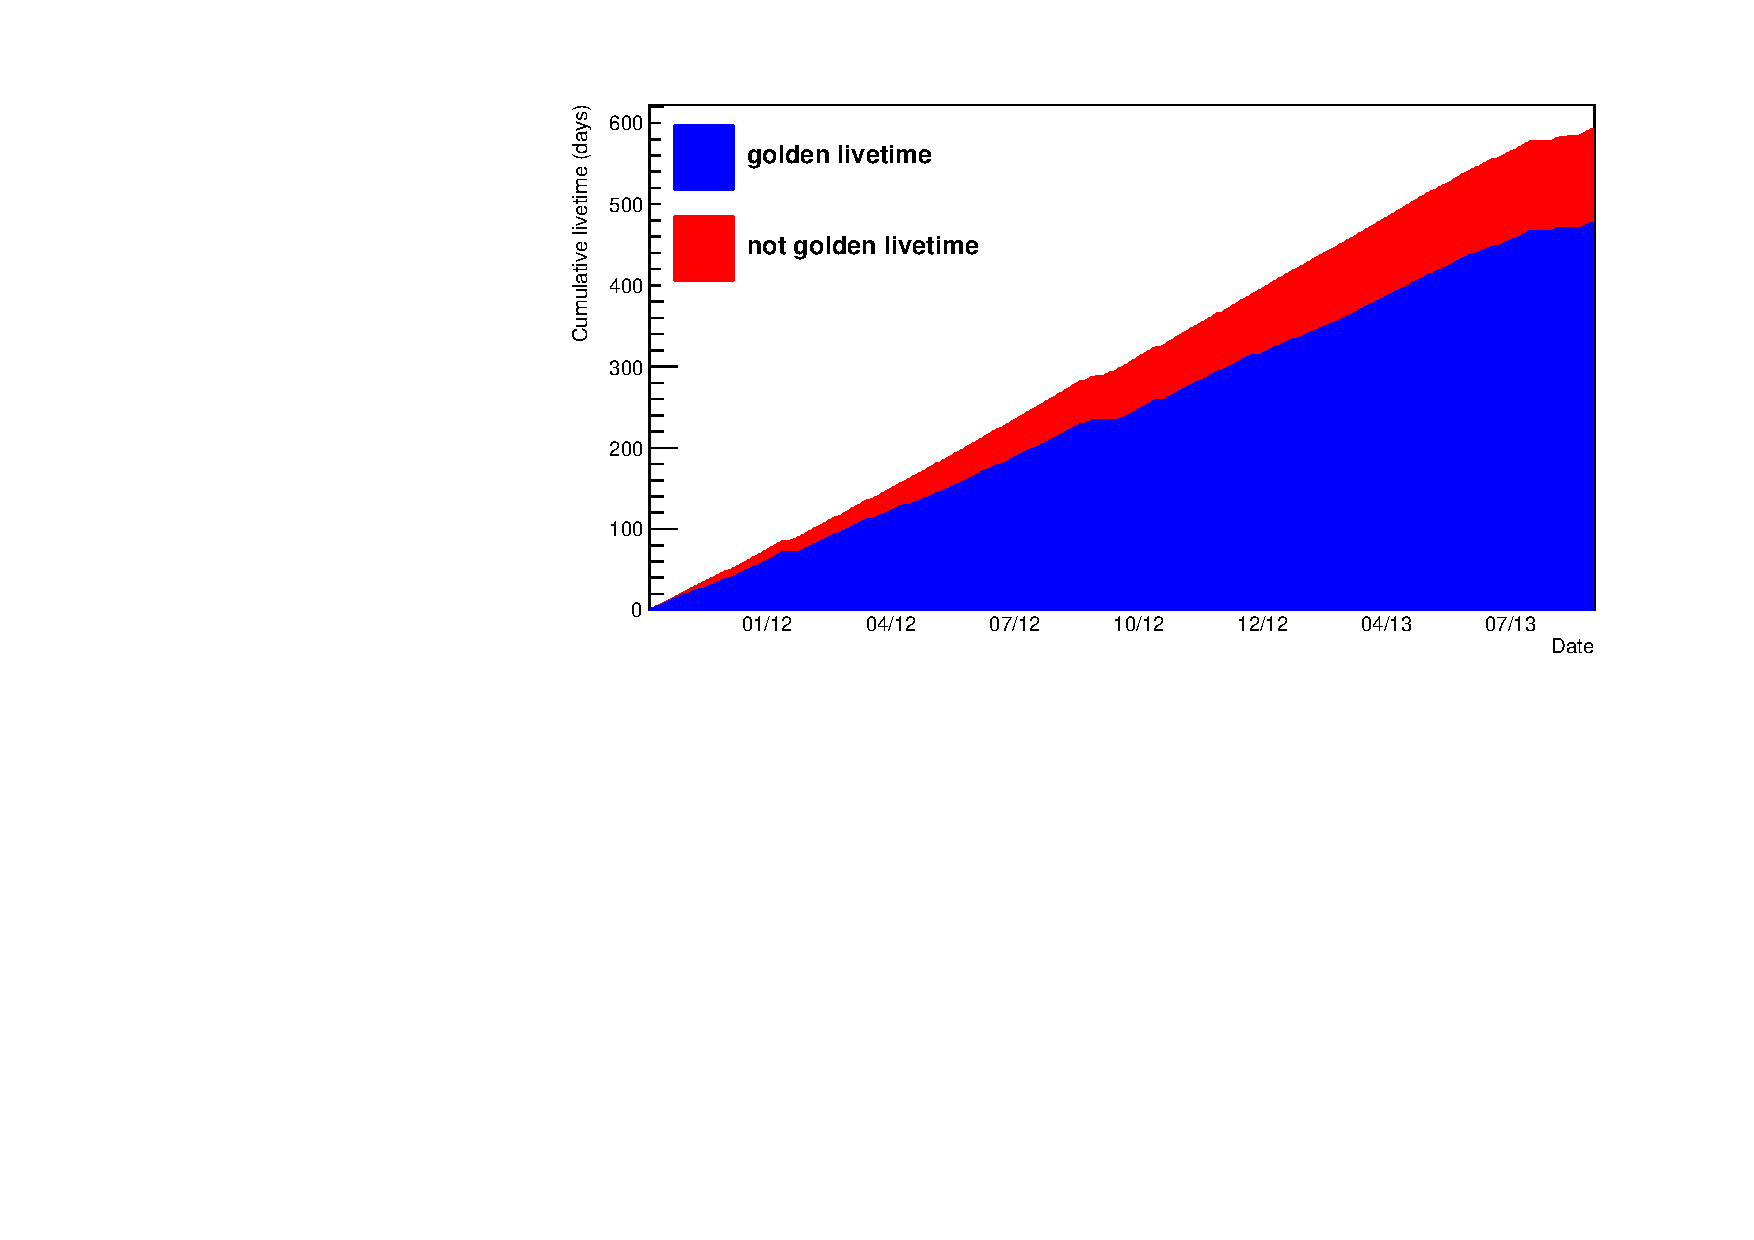
\includegraphics[keepaspectratio=true,width=\textwidth]{scripts/livetime.pdf}
\end{center}
\renewcommand{\baselinestretch}{1}
\small\normalsize
\begin{quote}
\caption{Cumulative low-background livetime collected in EXO-200.  Figure provided by David Auty.}
\label{fig:CumulativeLivetime}
\end{quote}
\end{figure}
\renewcommand{\baselinestretch}{2}
\small\normalsize

Although EXO-200 does occasionally take noise data, which consists of rapid requests for waveforms without any corresponding physics trigger, these runs have not been taken consistently throughout the EXO-200 dataset and will not be usable for measuring noise that changes over time.  However, during all low-background datataking it has been standard practice to request one trigger every ten seconds.  These solicited triggers, though infrequent, have cumulatively amounted to an enormous quantity of data which is expected to be purely noise.  Figure~\ref{fig:CumulativeLivetime} shows the cumulative low-background livetime which has been collected, and we can see that it is approximately evenly distributed across the dataset and, at a rate of $0.1$ Hz, millions of solicited triggers have been taken during the livetime of the detector.

The cuts we will make to select clean events are:
\begin{itemize}
\item Only golden-quality low-background runs (those deemed usable for final fits) will be used for noise measurements, to reduce the inclusion of anomalously noisy runs.
\item Events which occur during a ``bad'' time (times identified as anomalous within a run, eg. due to loud noises) are excluded.  Also, events occurring during the clean room siren are explicitly excluded, even though these times should generally also be marked as bad.
\item Only solicited-trigger events are used; events where a physics trigger fired may contain a pulse, regardless of what is found by reconstruction.
\item Truncated waveforms are not used, because they cannot provide the same set of noise frequencies as a full 2048-sample waveform.
\item Waveforms which saturate in any channel are not used.
\item Waveforms which are flagged as a known type of sporadic noise are excluded.
\item Events on which any u-wire or APD pulse was found by reconstruction are excluded.
\end{itemize}

From the set of acceptable events produced in this way, calculation of the noise correlation values is done in exactly the way implied by the definition of our noise correlation terms.  The expectation values are computed as averages over the set of events, so for example $\left<\widetilde{N}^R_i[f] \widetilde{N}^R_j[f]\right>$ is evaluated for a particular pair of channels $i$, $j$ and frequency index $f$ by computing $\widetilde{N}^R_i[f] \widetilde{N}^R_j[f]$ for all acceptable events, and then using the average of these values.  The symmetries of equations~\ref{eqn:NoiseSymmetryRRII} and \ref{eqn:NoiseSymmetryRIRI} are not currently used, but future versions of the code will exploit these symmetries to effectively double the number of independent measurements of each noise correlation.

The data are currently stored in a binary file as a sequence of eight-byte floating point numbers.  Binary portability has not been a serious concern because all machines on which the files are used have a similar architecture (little-endian, IEEE floating point format).  To studies of u-wire denoising, correlations are computed between all u-wire and APD channels, so the ordered list of channels is
\begin{equation}\label{eqn:ChannelListingForNoiseFile}
[0,1,2,...,36,37,76,77,...,112,113,152,153,...,225].
\end{equation}
No channel mapping is included in the file, so the set of included channels must be fixed regardless of the addition or subtraction of channels in the data (specifically, channel 163 and channel 16, both of which are only present in some of our data, and channels 178, 191, and 205, which were never active channels); these channels are included in the noise file, with noise fixed to zero where appropriate, and it is assumed that downstream software will be intelligent enough to use only those noise values which are meaningful.

The file stores noise correlations as a sequence of matrices, with one matrix for each frequency component except the baseline component $f = 0$.  We recall from equation~\ref{eqn:DefnOfCovarianceMatrix} that the covariance matrix of a list of random variables is defined as:
\begin{equation}
\mathbf{COV}\left( x_1, x_2, \dots, x_n \right) = \begin{pmatrix}
  cov(x_1, x_1) & cov(x_1, x_2) & \cdots & cov(x_1, x_n) \\
  cov(x_2, x_1) & cov(x_2, x_2) & \cdots & cov(x_2, x_n) \\
  \vdots & \vdots & \ddots & \vdots \\
  cov(x_n, x_1) & cov(x_n, x_2) & \cdots & cov(x_n, x_n)
\end{pmatrix}. \end{equation}
We recall that when $\left<x\right> = \left<y\right> = 0$, the covariance of random variables $x$ and $y$ will be simply $\left<xy\right>$; for us, all noise coefficients with $f > 0$ have mean zero.  For frequencies $0 < f < 1025$, we define an ordering for the electronic noise coefficients
\begin{equation}
\vec{\widetilde{N}}[f] = \left(\widetilde{N}^R_0[f], \widetilde{N}^R_1[f], ..., \widetilde{N}^R_{225}[f], \widetilde{N}^I_0[f], ..., \widetilde{N}^I_{225}[f]\right)
\end{equation}
where the channel index ranges over the channels listed in equation~\ref{eqn:ChannelListingForNoiseFile}.  For $f = 1025$ the imaginary components are all identically zero, so we define
\begin{equation}
\vec{\widetilde{N}}[1025] = \left(\widetilde{N}^R_0[1025], \widetilde{N}^R_1[1025], ..., \widetilde{N}^R_{225}[1025], \widetilde{N}^I_0[1025], ..., \widetilde{N}^I_{225}[1025]\right).
\end{equation}
Note that this is not the same as the index ordering used for computations in denoising and identified in equation~\ref{eqn:BlocksOfN}; since the on-disk format outlined here will need to be read into memory anyway, and since the list of channels on disk is different from the list of channels used for denoising, this is not a technical challenge but only a point which requires careful programming.

The binary-format noise file is then the sequence $\mathbf{COV}\left(\vec{\widetilde{N}}[1]\right)$, $\mathbf{COV}\left(\vec{\widetilde{N}}[2]\right)$, ..., $\mathbf{COV}\left(\vec{\widetilde{N}}[1025]\right)$, where each covariance matrix in turn is serialized to disk.  No current analysis requires baseline information, so the $f=0$ covariance matrix is omitted. Covariance matrices are symmetric, so the matrix serialization can be viewed equally well as column-major or row-major.  The matrices are all currently stored in unpacked format, meaning that no symmetries are currently exploited; future work should include specifying a more efficient packing of the noise coefficients which takes advantage of the symmetries described in section~\ref{sec:NoiseCorrelationsMath}.

Besides the anticipation of a change in file format in future versions of the code, there are other improvements to this algorithm which should be pursued in the future.  Some applications have been considered which would require knowledge of the noise on all channels, so the noise on v-wire channels should be recorded as well.  As another means of improving the usability of these files for other applications, an independent interface to the file format should be designed.  This could perhaps be written as a wrapper around some matrix serialization library, which could simplify the conversion between packed (for storage) and unpacked (for computation) symmetric matrix formats.

The highest priority, of course, will continue to be improving the quality of the noise correlations which are calculated.  Future topics for improvement are detailed in the next section.

\section{Future Directions with Noise Measurement}\label{sec:NoiseCorrelationsFuture}

Although the noise correlations described in this chapter have been sufficient for the present analysis, and there are no current indications that they are the limiting factor on denoising, still there are a number of possible improvements and extensions which could be investigated in future work.  Here we describe possible improvements to the quality of the noise correlations, followed by possible applications outside of denoising which may benefit from the use of noise correlations described in this chapter.

The general algorithm for creating noise correlations is fairly straightforward: identify time windows of constant noise behavior, select events within a noise window which appear to be clean representations of noise, and measure the average noise correlations (pairwise products) within those clean events.  However, there are potential improvements in all of these steps which may be subjects for future study.

For identifying the time windows, the current analysis is quite detailed in its attempt to correlate dramatic changes in noise behavior to known changes to the detector.  However, we have only begun to understand the more gradual changes to noise; one can imagine slow changes to noise on the order of weeks or months, or daily variations due to varying temperature, and neither would be well-captured by the current methods of identifying noise windows.  Combining charge injection noise and low-background noise studies should allow us to form a high-resolution map of the noise behavior over time, and it should be possible for us to understand exactly how stable the detector noise is over all time scales.  This is perhaps the most pressing need for future noise analysis.

\begin{figure}
\begin{center}
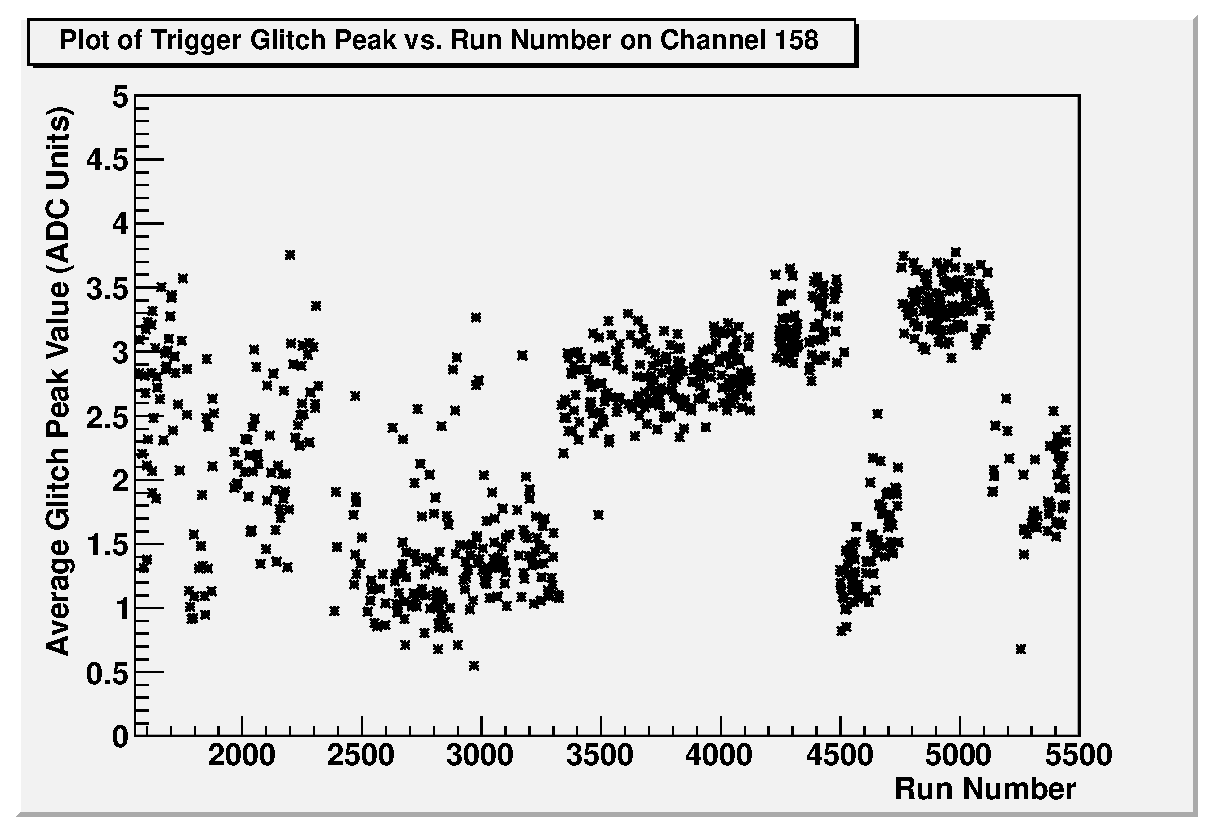
\includegraphics[keepaspectratio=true,width=\textwidth]{glitch_peak_vs_time_158.eps}
\end{center}
\renewcommand{\baselinestretch}{1}
\small\normalsize
\begin{quote}
\caption{The amplitude of the TEM injected pulses (``glitch'' pulses) over time for channel 158.  Figure provided by Sam Homiller.}
\label{fig:GlitchPeakAmplitudeVsTime}
\end{quote}
\end{figure}
\renewcommand{\baselinestretch}{2}
\small\normalsize

The selection of clean events is also a topic requiring further study.  Although solicited triggers are treated as clean events, it has long been known that the TEM can inject pulses into events during solicited triggers; the mechanism by which it does so is unknown.  This injected pulse is correlated with the trigger time, meaning that it has a non-random phase; Sam Homiller has made a preliminary study to separate the injected pulses from noise by exploiting this property of non-random phase, and the amplitudes of these pulses over time for a particular channel are shown in figure~\ref{fig:GlitchPeakAmplitudeVsTime}.  In the present analysis these injected pulses are assumed to be small and ignored.  However, the tools to subtract the mean injected pulses have already been developed, and we should investigate:
\begin{itemize}
\item Do injected pulses occur with all trigger types, or only solicited triggers?
\item Does subtraction of injected pulses improve the quality of the noise correlations or the results from denoising?
\end{itemize}

Finally, section~\ref{sec:NoiseCorrelationsMath} described how we neglect the possible aliasing of extremely low-frequency noise.  To a first approximation this would simply be observed as a drift in the baseline of waveforms, which has no significant effect on the offline analysis (though it may have an impact on the online triggering threshold).  However, a more accurate treatment may observe that low-frequency noise is aliased into the low Fourier components with $f = 0, 1, 2, ...$ in a way which does not accurately reflect the true noise in the detector.  Such aliasing would perhaps lead to an event-by-event bias in reconstructed peak magnitudes, both from standard reconstruction and denoising.  It may be possible to estimate the contribution from aliasing by looking for periodicity in the low frequency Fourier components event-by-event; noise runs (such as run 4796, a ten-minute 50-Hz solicited trigger run taken under normal running conditions) would be a particularly good place to look for such an effect because of the higher rate of usable noise events in that data.  One approach to combining many events into a single estimate of noise frequency components that extends to lower frequency could be to use a non-equispaced Fourier transform~\cite{Keiner:2009:UNS:1555386.1555388}.

Another extension of the current work with noise correlations, related to the question of whether aliasing is a significant effect, is to study whether we can interpolate from the noise correlations of a 2048-sample waveform what the expected noise correlations for a shorter (truncated) waveform would be.  Generally, it is expected that the longer a waveform is, the more information it will provide; so it should be true that a 2048-sample noise waveform provides more information than a truncated waveform provides.  We would like to be able to downsample the noise correlations from a 2048-sample waveform to the expected noise correlations for a truncated waveform on this premise.  However, if aliasing is a significant factor then it may be that the low-frequency aliasing observed in a 2048-sample waveform is different from the aliasing observed in a truncated waveform, and it may be that a simple interpolation of the 2048-sample noise correlations is not an accurate reflection of the noise observed on truncated waveforms.  (Conversely, it may be that truncated waveforms are more vulnerable to low-frequency aliasing than 2048-sample waveforms; in this case it may be that the downsampled noise from a 2048-sample waveform is an accurate reflection of noise on the truncated waveform, but that the Fourier transform of the shorter waveform still exhibits too much aliasing to be usable.)  Understanding the degree to which we can understand noise on truncated waveforms and evade low-frequency aliasing issues for truncated waveforms would be a key step to understanding whether denoising can be extended to operate on such events.

It may also be hoped that these noise correlations will find uses beyond denoising and other signal processing applications.  One example which is currently under consideration is for simulated noise.  It is a general observation within EXO-200 that the noise model employed in our simulations is simple, ignoring all correlations and all noise frequency peaks which have been observed in data.  For many purposes this is sufficient, but to fully model our energy threshold a more accurate model is needed.  Preliminary investigations have focused on sampling noise directly from the observed waveforms and using these noise samples, as described in section~\ref{sec:ResultsDigitization}.  However, it would also be possible to use the noise correlations described in this chapter to represent our most complete understanding of the noise in the detector, and simulate noise which matches those noise correlations.  This can be accomplished by computing the Cholesky decomposition of the noise correlations, viewed as a covariance matrix, as described in~\cite{ross2012simulation}.

This chapter has described the measurement of electronic noise correlations from low-background data, with significant input from charge injection runs as well.  Noise is one of the central features of the EXO-200 analysis, and understanding it in detail is a critical component to an effective denoising strategy.  Thus, the result of this chapter can be understood as one of the two key inputs to denoising.  The other, the APD lightmap, is described in chapter~\ref{ch:Lightmap}.
